\chapter {Literature Review}
\label{literature_review}
The From segmentation process is related to edge ditection, finding contours and contours shapes,and text ditection related to Tesseract and Tesseact training. Thus in this chapter we will discuss about some state of the art image processing techniques and Tesseract OCR applications.
\section{Canny Edge Ditection}
\label{EdgeDitectionR}
The Canny edge detector is an edge detection operator that uses a multi-stage algorithm to detect a wide range of edges in images. It was developed by John F. Canny in 1986. Canny also produced a computational theory of edge detection explaining why the technique works \cite{EdgeDetection} \cite{CannyEdgeDetection3}.
\subsection{Canny Edge Ditection Algorithm}
Canny edge detection algorithm go through these following steps:
\begin{enumerate}
\item In order to implement the canny edge detector algorithm, a series of steps must be followed. The first step is to filter out any noise in the original image before trying to locate and detect any edges. And because the Gaussian filter can be computed using a simple mask, it is used exclusively in the Canny algorithm. Once a suitable mask has been calculated, the Gaussian smoothing can be performed using standard convolution methods. A convolution mask is usually much smaller than the actual image. As a result, the mask is slid over the image, manipulating a square of pixels at a time. The larger the width of the Gaussian mask, the lower is the detector's sensitivity to noise. The localization error in the detected edges also increases slightly as the Gaussian width is increased. The Gaussian mask used in my implementation is shown below. 

\begin{figure}[H]
\centering
\label{fig:GaussainMask} 
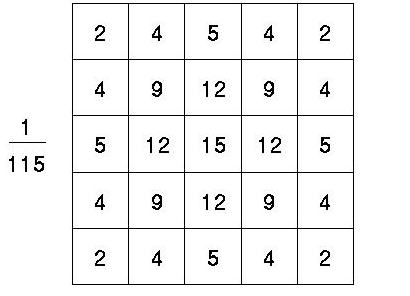
\includegraphics[width=0.5\textwidth]{GaussMask}
\caption {Discrete Approximation to Gaussian function with $\sigma = 1.4$}
\end{figure}


\item After smoothing the image and eliminating the noise, the next step is to find the edge strength by taking the gradient of the image. The Sobel operator performs a 2-D spatial gradient measurement on an image. Then, the approximate absolute gradient magnitude (edge strength) at each point can be found. The Sobel operator uses a pair of 3x3 convolution masks, one estimating the gradient in the x-direction (columns) and the other estimating the gradient in the y-direction (rows). They are shown below:
\begin{figure}[H]
\centering
\label{fig:Mask} 
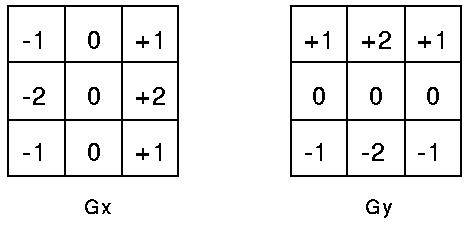
\includegraphics[width=0.6\textwidth]{Mask}
\end{figure}
The magnitude, or EDGE STRENGTH, of the gradient is then approximated using the formula: $|G| = |Gx| + |Gy|$
\item Finding the edge direction is trivial once the gradient in the x and y directions are known. However, you will generate an error whenever sumX is equal to zero. So in the code there has to be a restriction set whenever this takes place. Whenever the gradient in the x direction is equal to zero, the edge direction has to be equal to 90 degrees or 0 degrees, depending on what the value of the gradient in the y-direction is equal to. If GY has a value of zero, the edge direction will equal 0 degrees. Otherwise the edge direction will equal 90 degrees. The formula for finding the edge direction is just: $$\theta = tan^{-1} (Gy / Gx)$$

\item Once the edge direction is known, the next step is to relate the edge direction to a direction that can be traced in an image. So if the pixels of a 5x5 image are aligned as follows: \\
\begin{table}[H]
\centering
\begin{tabular}{|c c c c c|}
\hline
x & x & x & x & x \\
x & x & x & x & x \\
x & x & x & x & x \\
x & x & \textcolor{red}{a} & x & x \\
x & x & x & x & x \\
x & x & x & x & x \\
\hline
\end{tabular}
\caption {Edge Ditection}
\label {tab:Table1}
\end{table} 
Then, it can be seen by looking at pixel "\textcolor{red}{a}", there are only four possible directions when describing the surrounding pixels - 0 degrees (in the horizontal direction), 45 degrees (along the positive diagonal), 90 degrees (in the vertical direction), or 135 degrees (along the negative diagonal). So now the edge orientation has to be resolved into one of these four directions depending on which direction it is closest to (e.g. if the orientation angle is found to be 3 degrees, make it zero degrees). Think of this as taking a semicircle and dividing it into 5 regions.
\begin{figure}[H]
\centering
\label{fig:Canny1} 
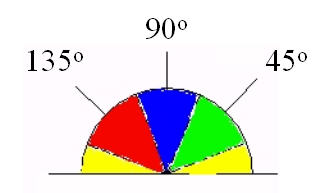
\includegraphics[width=0.6\textwidth]{Canny}
\end{figure}
Therefore, any edge direction falling within the \textcolor{yellow}{yellow range} (0 to 22.5 \& 157.5 to 180 degrees) is set to 0 degrees. Any edge direction falling in the \textcolor{green}{green range} (22.5 to 67.5 degrees) is set to 45 degrees. Any edge direction falling in the \textcolor{blue}{blue range} (67.5 to 112.5 degrees) is set to 90 degrees. And finally, any edge direction falling within the \textcolor{red}{red range} (112.5 to 157.5 degrees) is set to 135 degrees.
\item After the edge directions are known, nonmaximum suppression now has to be applied. Nonmaximum suppression is used to trace along the edge in the edge direction and suppress any pixel value (sets it equal to 0) that is not considered to be an edge. This will give a thin line in the output image.
\item Finally, hysteresis is used as a means of eliminating streaking. Streaking is the breaking up of an edge contour caused by the operator output fluctuating above and below the threshold. If a single threshold, T1 is applied to an image, and an edge has an average strength equal to T1, then due to noise, there will be instances where the edge dips below the threshold. Equally it will also extend above the threshold making an edge look like a dashed line. To avoid this, hysteresis uses 2 thresholds, a high and a low. Any pixel in the image that has a value greater than T1 is presumed to be an edge pixel, and is marked as such immediately. Then, any pixels that are connected to this edge pixel and that have a value greater than T2 are also selected as edge pixels. If you think of following an edge, you need a gradient of T2 to start but you don't stop till you hit a gradient below T1. \cite{CannyEdgeDetection1}\cite{CannyEdgeDetection2}
\end{enumerate}
\section{Contours}
Contours can be explained simply as a curve joining all the continuous points (along the boundary), having same color or intensity. The contours are a useful tool for shape analysis and object detection and recognition. \cite{Contours}
\begin{itemize}
\item For better accuracy, use binary images. So before finding contours, apply threshold or canny edge detection.
\item findContours function modifies the source image. So if you want source image even after finding contours, already store it to some other variables.
\item In OpenCV, finding contours is like finding white object from black background. So remember, object to be found should be white and background should be black.
\end{itemize}
\begin{figure}[H]
\centering
\subfloat [Original Image]{\label{fig:Contour2} 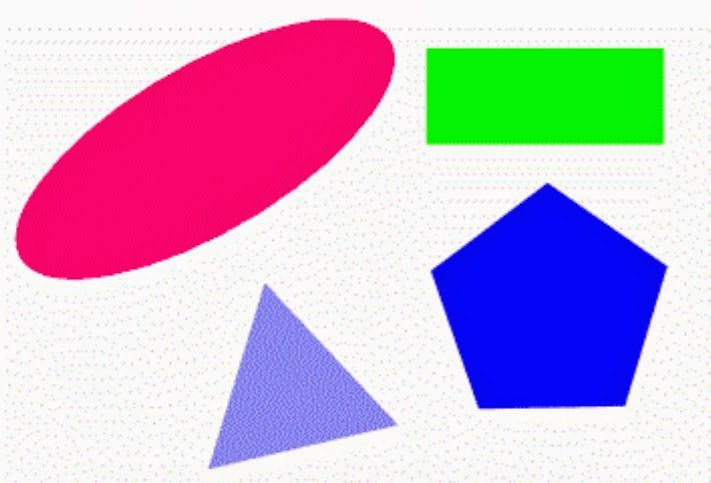
\includegraphics[width=0.5\textwidth]{shape.JPG}}
\subfloat [Detected Contours]{\label{fig:DetectContour} 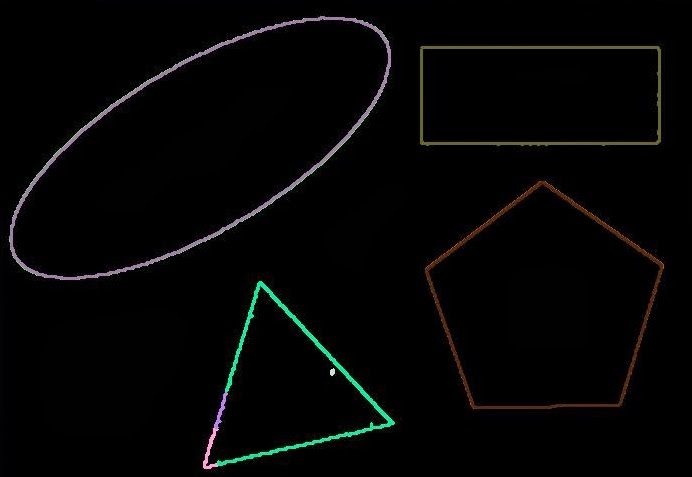
\includegraphics[width=0.5\textwidth]{contours.JPG}}
\caption {Find Courours}
\label {fig:Amino_Acid}
\end{figure}
\section{Detecting shapes in images}
\label{Shape}
Doing image processing and especially blob analysis it is often required to check some objects' shape and depending on it perform further processing of a particular object or not. For example, some applications may require finding only rectangle from all the detected objects, or quadrilaterals, rectangles, etc.
\subsection{Detection quadrilaterals}
Detection of quadrilaterals and triangles has pretty much the same idea - we are checking mean distance between provided shape's edge pixels and the edge of estimated quadrilateral/triangle. The only difference here is the way how to estimate parameters of the shape we want to recognize and how to check distance to the estimated shape.

Let's start with quadrilaterals first. For a given shape we can make an assumption that it is a quadrilateral, find its four corners and then using similar method as we've used for circles we can check if our assumption is correct or not - check how good the shape fits into the quadrilateral with assumed parameters.
\begin{figure}[H]
\centering
\label{fig:shape} 
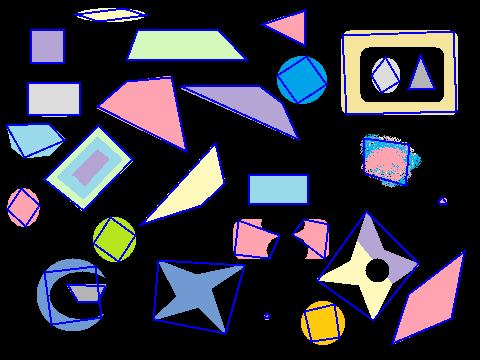
\includegraphics[width=0.6\textwidth]{shapefourcorner}
\caption {Detection of quadrilaterals}
\end{figure}
As we can see on the image above, we may have different objects and quadrilateral finder provides different results for them. For shapes which really look like quadrilateral, the quadrilateral finder is able to find their corners more or less correctly (problem may occur in the case if object has rounded corners). But for other types of objects (circles, starts, etc.), quadrilateral finder does not provide any good result. And this is correct, since this routine supposes the given shape is really quadrilateral.

Now, when we made the assumption that a subjected object is quadrilateral and we got its corner, we just need to see how good is the fit of the object into the quadrilateral with those found corner - we need to make sure there are no edge points of the given shape which are too far away from the edge of the assumed quadrilateral.
\subsection{Detection Rectangles, squares, equilateral}
Once we made a check for quadrilateral shape and got its 4 corners, we may do some further checks to detect sub-type of the quadrilateral: trapezoid, parallelogram, rectangle, rhombus or square. These checks are based on checking angles between opposite/adjacent sides and their length. First we check two opposite sides - if they are parallel, then we get at least trapezoid. Then we check two other sides - if they are parallel two, then we have parallelogram. If two adjacent sides are perpendicular, then we got rectangle. The last check is to compare length of two adjacent sides - if they are equal, then parallelogram becomes rhombus and rectangle becomes square. And of course we need to add small possible error, so if angle between lines equals to 2 degrees, they are still treated as parallel. \cite{DetectingShape}
\section{Tesseract OCR Engine}
\subsection{What is Tesseract?}
An Overview of the Tesseract OCR Engine describes Tesseract as: "Tesseract is an open source
optical character recognition(OCR) engine. HP originally was originally started it as a project. Later it was modified, improved and taken over by Google and later released as open source
in year 2005. It is now available at" (Smith, 2007) . It is very portable as compared to others
and supports various platforms. Its focus is more towards providing less rejection and improved
accuracy. Currently only command base version is available but there are many projects with UI
built on top of it which could be forked. As of now Tesseract version 3.02 is released and
available for use. Now Tesseract is developed and maintained by Google. It provides support for
around 139 languages \cite{TesseractORCEngine}.
\subsection{Architecture}
Tesseract OCR is an elegant engine with various layers. It works in step by step manner as
shown in the block diagram in fig 3.4. The first step in the cycle is to sense the color intensities of the image, named as adaptive thresholding, and converts the image into binary images.
Second step is to do the connected component analysis of the image, which does the task of
extracting character outlines. This step is the main process of this cycle as it does the OCR of
image with white text and blacks rest of the image.
Tesseract was probably the first to use these cycles to process the input image. After this the
outlines extracted from image are converted into Blobs(Binary Long Objects). It is then organized as lines and regions and further analysis is for some fixed area. After extraction
the extracted components are chopped into words and delimited with spaces. Recognition in text
then starts which is a two pass process. As shown in fig 1, the first part is when attempt to
recognize each word is made. Each satisfactory word is accepted and second pass is started to
gather remaining words. This brings in the role of adaptive classifier. The adaptive classifier then will classify text in more accurate manner. The adaptive classifier needs to be trained beforehand
to work accurately. When the classifier receives some data, it has to resolve the issues and assign
the proper place of the text\cite{TesseractORCEngine} \cite{TesseractORCEngine2}.

\begin{figure}[H]
\centering
\label{flow} 
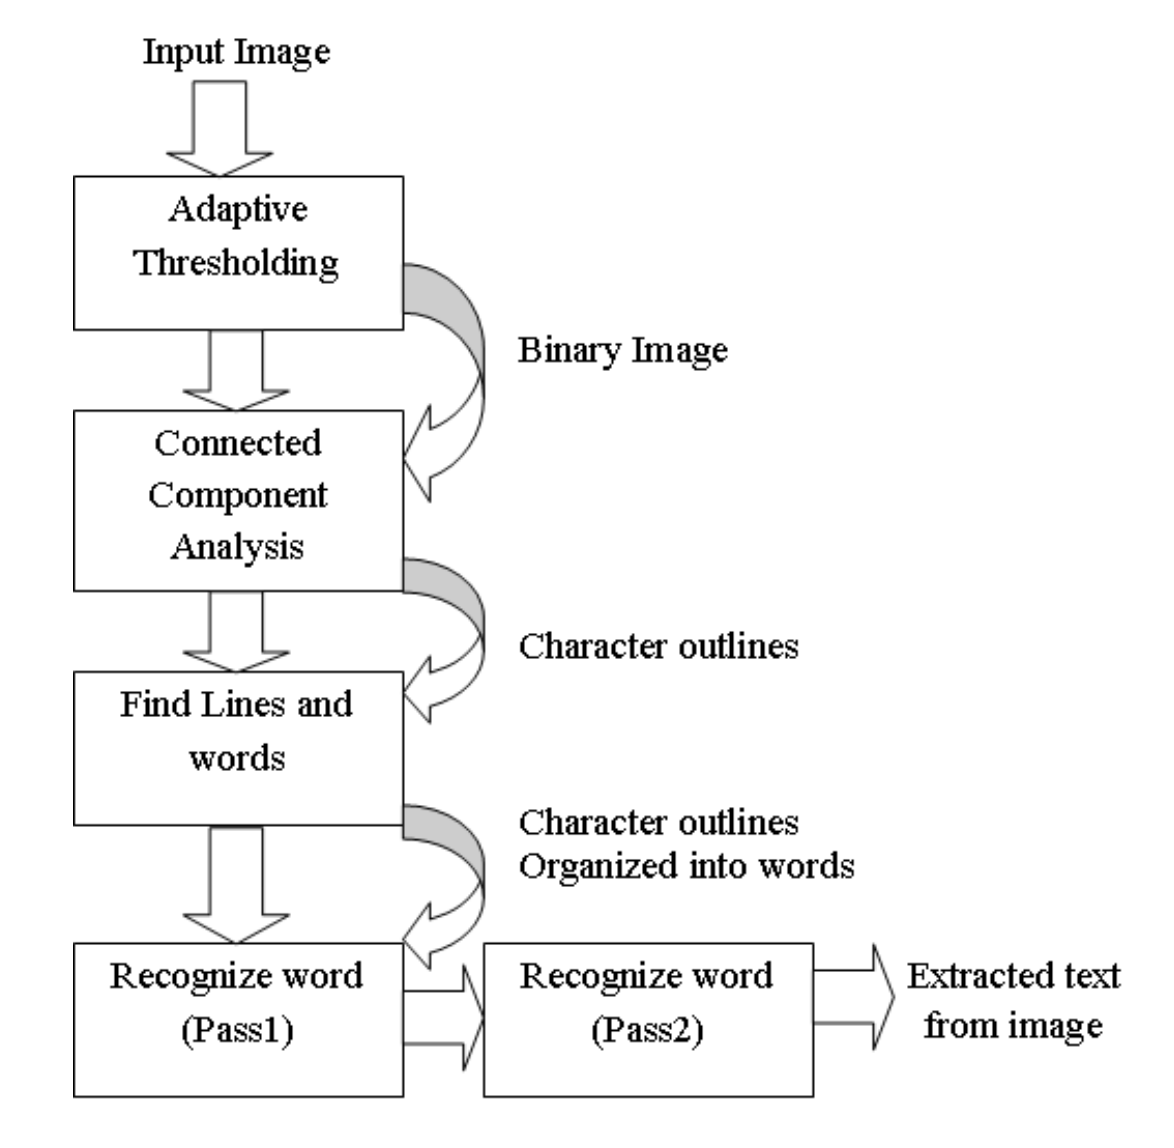
\includegraphics[width=0.8\textwidth]{tesseractFlow}
\caption {Tesseract Flow}
\end{figure}

\subsection{Working of Tesseract}
Tesseract works pretty much as a scanner. Its interface is pretty simple as it takes input o the command lines with very basic commands. We need to input any image with text in it.

The basic Tesseract command takes only two arguments: First is input image that contains text and second argument is output text file which is usually text file.

Tesseract by default picks the extension of output file as .txt. There no need to specify the explicitly the output file extension.Tesseract supports various languages. Each language comes with a trained language data file.

The language file must be kept in a location Tesseract knows. When using in the project it is advised to keep it within the project folder. This folder is Tesseract home folder in your machine. In this research, we are aiming to extract English and Bangla characters from the images so we have to keep both Bangla and English data files \cite{TesseractORCEngine}.
 
\subsection{How does Tesseract work?}
\textbf{The following is a brief overview of how Tesseract works\cite{TesseractORCEngineOfficialWeb}:}
\begin{enumerate}
\item Outlines are analysed and stored 
\item Outlines are gathered together as Blobs
\item Blobs are organized into text lines
\item Text lines are broken into words 
\item First pass of recognition process attempts to recognize each word in turn 
\item Satisfactory words passed to adaptive trainer 
\item Lessons learned by adaptive trainer employed in a second pass, which attempts
recognize the words that were not recognized satisfactorily in the first pass 
\item Fuzzy spaces resolved and text checked for small caps
\item Digital texts are outputted 
\end{enumerate}
\textbf{During these processes, Tesseract uses:}
\begin{enumerate}
\item algorithms for detecting text lines from a skewed page 
\item algorithms for detecting proportional and non proportional words (a proportional
word is a word where all the letters are the same width) 
\item algorithms for chopping joined characters and for associating broken characters 
\item linguistic analysis to identify the most likely word formed by a cluster of
characters 
\item two character classifiers: a static classifier, and an adaptive classifier which
employs training data, and which is better at distinguishing between upper and
lower case letters 
\end{enumerate}

\subsection{Limitations of Tesseract}
\textbf{Tesseract is an OCR engine, not a complete OCR program.\cite{TesseractORCEngineOfficialWeb}}
Tesseract is an OCR engine rather than a fully featured program similar to commercial
OCR software such as Nuance’s Omnipage. It was originally intended to serve as a
component part of other programs or systems. Although Tesseract works from the 
command line, to be usable by the average user the engine must be integrated into
other programs or interfaces, such as FreeOCR.net, WeOCR or OCRpous. Without
integration into programs such as these, Tesseract has no page layout analysis, no
output formatting and no graphical user interface (GUI).

\section{Training Tesseract}
The setup for English \& Bangla OCR within Tesseract is another important task. The way train the engine and input the dataset matters a lot\cite{TesseractTrain}\citep{hasnat2009open}.
Training Tesseract for English \& Bangla includes four steps mainly and they are as follows:
\subsection{Generating training images}
Tesseract official website explains these steps very well "The first step is to determine the full
character set to be used, and prepare a text or word processor file containing a set of examples". The two important points to remember for a training file are: Firstly make sure the file
contains all the characters that we are expecting. Secondly there should be at least 5 samples.
There should be more samples of the more frequent characters - at least 20. Keeping all this
in mind let's explore how do we create box files \cite{TesseractTrain}.
\subsection{Make box files}
Box file is defined as a sample to match with the characters. We need a 'box' file for each
training image. Tesseract official website defines the box file as "The box file is a text file that
lists the characters in the training image, in order, one per line, with the coordinates of the
bounding box around the image". Tesseract is not so intuitive about the sample data.
Inconsistencies may lead to wrong interpretation of data\cite{TesseractTrain}.
\subsection{Run Tesseract}
In this step we run the Tesseract engines with the new training files. The purpose is to create the
trained dataset which works as a rule engine. Also it creates log files\cite{TesseractTrain}.
\subsection{Compute character set} 
Guidelines from Tesseract website state that "Tesseract needs to know the set of possible characters it can output. To generate the unichar set data file, use the unicharset\textunderscore extractor program on the box files generated above":extractor language. fontname. box 
One more requirement in this is, Tesseract needs to have access to character properties i.e.
isalpha, isdigit, isupper, islower, ispunctuation.
The system described in have classified Hindi OCR and its setup, training very nicely.
The only limitation is that the system is for desktop. We have to build the similar system for
mobile devices.\cite{TesseractTrain}
\section{OpenCV}
OpenCV (Open Source Computer Vision) is a library of programming functions and algorithms. Their main focus is to provide API mainly aimed at real-time computer vision. It was
originally developed by Intel. OpenCV library is free for use for development (under the open
source BSD license). The best feature is that the library is cross-platform . \cite{TesseractTrain}